\documentclass[12pt]{article}
\usepackage[utf8]{inputenc}
\usepackage[a4paper,top=2.5cm,bottom=2.5cm,left=2cm,right=2cm]{geometry}
\usepackage{amsmath}
%\usepackage{upgreek}
\usepackage{enumerate}
\usepackage{indentfirst}
\usepackage{subcaption}
\usepackage{graphicx}
\usepackage{caption}
\usepackage{siunitx}
\usepackage{array}
\usepackage{multirow}

\setlength{\parindent}{4ex}

\title{Test File 2}
\author{author's name}
\date{}

\begin{document}
\maketitle

\begin{figure}[!h]
\centering
  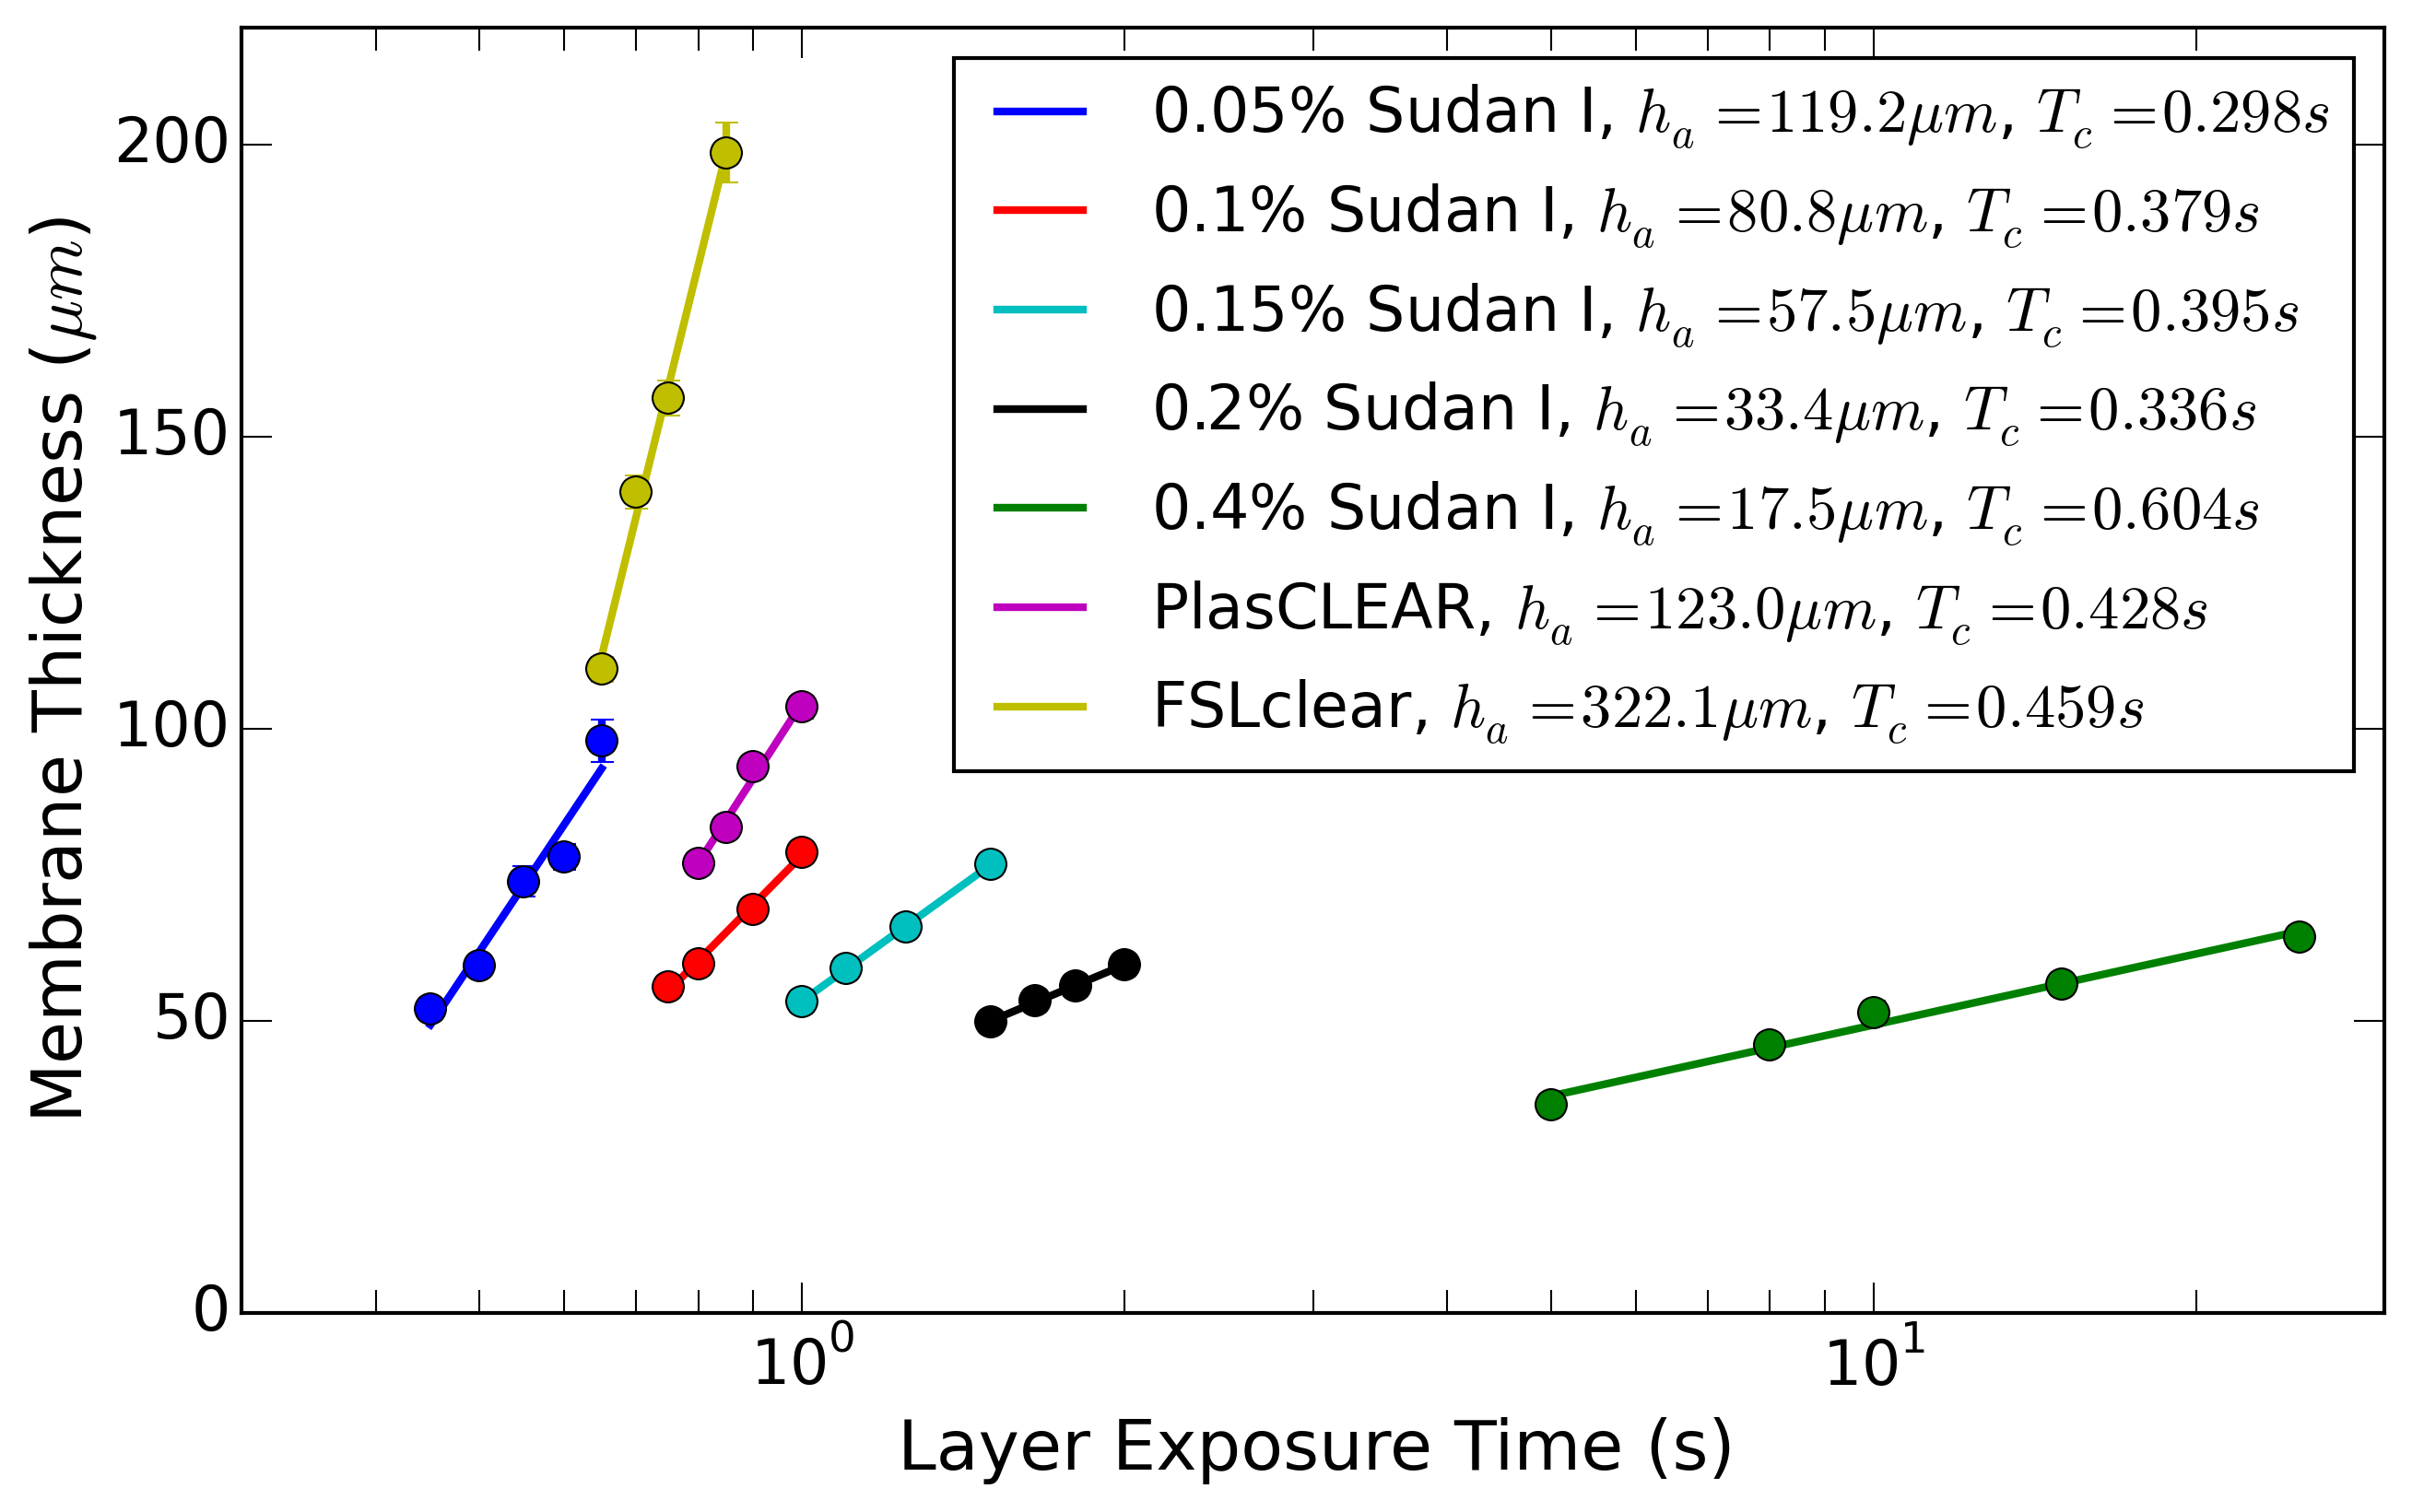
\includegraphics[width=0.5\textwidth]{ha_Tc.png}
  \caption{Measured $h_a$ and $T_c$ of different resins. }
  \label{fig:ha_Tc}
\end{figure}

In Fig. \ref{fig:ha_Tc}, the $h_a$ and $T_c$ are also listed, which correspond to the absorbance memsured in Fig. \ref{fig:spectra}. To further confirm our model, the measured $h_a$ and $T_c$ are employed to calculate the required exposure time for a 10 $\mu$m membrane for 0.2\% Sudan I resin, and it is 0.45 s. The printed membrane is given in Fig. \ref{fig:10um_memb}, measured about 10 $\mu$m.

\end{document}